\documentclass{article}
\usepackage[utf8]{inputenc}
\usepackage{graphicx}
\usepackage{titlepic}
\usepackage{caption}
\usepackage{subcaption}
\usepackage{listings}
\usepackage{color}
\usepackage{amsmath}
\usepackage{float}
% \documentclass{beamer}

\newcommand{\namesigdate}[2][5cm]{%
  \begin{tabular}{@{}p{#1}@{}}
    #2 \\[0.4\normalbaselineskip] \hrule \\[0pt]
    {\small } \\[2\normalbaselineskip] 
  \end{tabular}
}
%New colors defined below
\definecolor{codegreen}{rgb}{0,0.6,0}
\definecolor{codegray}{rgb}{0.5,0.5,0.5}
\definecolor{codepurple}{rgb}{0.58,0,0.82}
\definecolor{backcolour}{rgb}{0.95,0.95,0.92}

%Code listing style named "mystyle"
\lstdefinestyle{mystyle}{
  backgroundcolor=\color{backcolour},   commentstyle=\color{codegreen},
  keywordstyle=\color{magenta},
  numberstyle=\tiny\color{codegray},
  stringstyle=\color{codepurple},
  basicstyle=\footnotesize,
  breakatwhitespace=false,         
  breaklines=true,                 
  captionpos=b,                    
  keepspaces=true,                 
  numbers=left,                    
  numbersep=5pt,                  
  showspaces=false,                
  showstringspaces=false,
  showtabs=false,                  
  tabsize=2
}

\lstset{style=mystyle}

\title{\vspace*{\fill} \textbf{3D reconstruction using an IMU enabled mobile device}
	  \\ {\large \textbf{Summer Undergraduate Research Award}}
	  \\  \vspace{3mm} 
\includegraphics[width=5cm]{logo.png}}

\author{
	\textbf{Kartikeya Gupta}\\ 
	2013CS10231\\
	Computer Science\\
	CGPA: 9.78 \\
	Mob: 9899134337\\
	cs1130231@iitd.ac.in
	\and
	\textbf{Prateek Kumar Verma}\\ 
	2013CS10246\\
	Computer Science\\
	CGPA: 8.87\\
	Mob: 9911577289\\
	cs1130246@iitd.ac.in
}
\date{\textbf{Supervisor:-} \\ \textbf{Subhashis Banerjee} \\ Professor \\ Department of CSE \\ suban@cse.iitd.ac.in\\ IIT Delhi\\
\vspace*{\fill}}




\begin{document}
		% 
\includegraphics{logo.png}

% \noindent \namesigdate{} \hfill \namesigdate[3cm]{Saroj Kaushik \\ HOD CSE }
% \begin{flushleft}
% \noindent \namesigdate{} 
% \end{flushleft}



% \begin{flushright}
% \noindent\rule{3.2cm}{0.4pt} 
% \\ \textbf{Prof. Saroj Kaushik}
% \\ Head of Department
% \\ Department of CSE
% \\ saroj@cse.iitd.ernet.in
% \end{flushright}


	\newpage
	% \begin{figure}
% \end{figure}
	
	\section{Introduction}
		\textit{\textbf{3D reconstruction}} is the process of capturing the shape and appearance of real objects. The conventional methods for 3D reconstruction is based on \textit{multiple images}. In this method, 3D models are constructed from a set of images. It can be considered as a reverse process of obtaining 2D images from 3D scenes.
		\newline
		3D reconstruction has a wide variety of applications. It allows engineers and students to work more efficiently as they can generate copies of 3D objects easily. In orthopedics and joint replacement surgery, the complicated parts to be replaced can be made with high accuracy. Also, it can be used to generate replica of artifacts and fragile objects for further studies, without harming its integrity.

		\begin{figure}[ht!]
			\centering
			\begin{subfigure}{.5\textwidth}
			  	\centering
			  	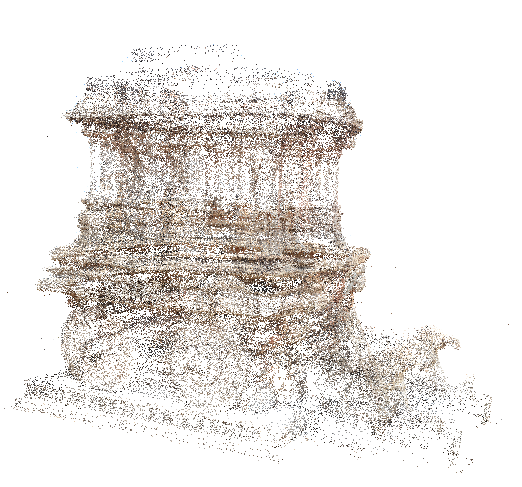
\includegraphics[width=1.0\linewidth]{sparse_chariot.png}
			  	\caption{Sparse reconstruction}
			  	\label{fig:sub1}
			\end{subfigure}%
			\begin{subfigure}{.5\textwidth}
			  	\centering
			  	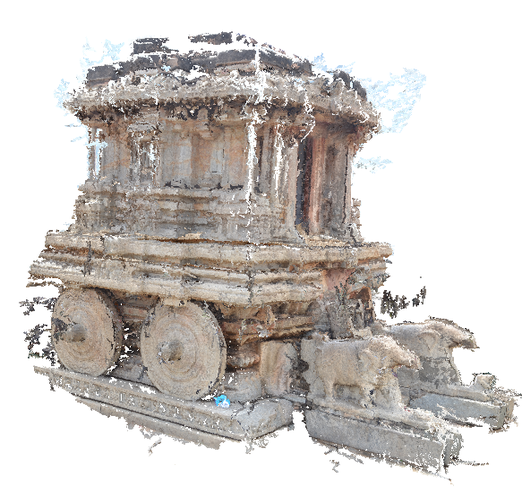
\includegraphics[width=1.0\linewidth]{dense_chariot.png}
			  	\caption{Dense reconstruction}
			  	\label{fig:sub2}
			\end{subfigure}
			\caption{3D reconstruction}
			\label{figstart}
		\end{figure}


		Figure~\ref{fig:sub1} shows the first step towards 3D construction i.e. \textit{Sparse reconstruction}, which is done for some set of points. Figure~\ref{fig:sub2} is the final reconstructed 3D model of the object. The \textit{traditional pipeline} is shown in Figure~\ref{fig3}.

		\begin{figure}[ht!]
		\centering
		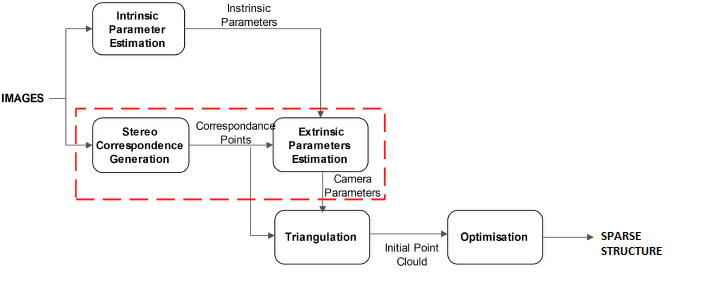
\includegraphics[width=14cm]{traditional_pipeline2.png}
		\caption{Traditional pipeline\label{fig3}}
		\end{figure}

		The red-highlighted part of the pipeline is \textit{\textbf{computationally expensive}}. Thus, our project aims to reduce this computation and perform 3D reconstruction in near real-time.

		The processing parts are:
			\begin{itemize}
			\item \textit{Intrinsic and extrinsic parameters}: The camera projection matrix is a $3 \times 4$ matrix which represents the pinhole geometry of a camera for mapping 3D points in the world coordinates to 2D points on images. This matrix depends on extrinsic and intrinsic parameters. The intrinsic parameters mainly comprises of focal length, image sensor format, and principal points. The extrinsic parameters define the position of the camera center and the camera's heading in world coordinates in terms of a rigid rotation and translation. 
			\item \textit{Stereo correspondence generation}: Given two or more images of the same 3D scene, taken from different points of view, the correspondence problem refers to the task of finding a set of points in one image which can be identified as the same points in another image. To do this, points or features in one image are matched with the corresponding points or features in another image. The images can be taken from a different point of view, at different times, or with objects in the scene in general motion relative to the camera(s).
			\item \textit{Triangulation}: Triangulation refers to the process of determining a point in 3D space given, its projections onto two or more images and their corresponding camera projection matrices. This point is found as the intersection of the two or more projection rays formed from the inverse projection of the 2D image points representing that 3D point in space.
			\item \textit{Initial point cloud and 3D sparse reconstruction}: As the word suggests, \textit{3D sparse construction} is done for only some set of data points in the given coordinate system called \textit{initial point cloud}. Figure~\ref{fig:sub1} illustrates a 3D sparse construction of a chariot. Figure~\ref{fig:sub2} illustrates 3D dense construction of the same initial point cloud.

			\end{itemize}
	
\section{Basic Concepts} 
		%\begin{itemize}
			\subsection{Camera calibration}
				The camera parameters can further be subdivided into intrinsic and extrinsic parameters. \textbf{Camera intrinsic parameter} $K$ is dependent on the focal length of the camera and principal point (which in most cases is the center of the image). The \textbf{camera extrinsic parameter} is composed of the rotation $R$ and translation $t$ between camera coordinate system and the world coordinate system. Together they form the camera projection matrix $P$, a $3 \times 4$ matrix which describes the mapping of a pinhole camera from 3D points in the world to 2D points in an image.
				\begin{equation}
				P = K[R|t]
				\end{equation}
			
			\subsection{Sparse 3D reconstruction} 
				Given two different images of the same scene from different angles, the position of a 3D point can be found as the intersection of the two projection rays which is commonly referred to as \textbf{triangulation}. For this first point correspondences have to be established. Then using this point correspondences a Random Sampling Consensus (RANSAC) based voting framework is used to estimate the camera intrinsic and extrinsic parameters. Finally, a joint non-linear optimization is used to further refine the camera parameters and the 3D points in a \textbf{bundle adjustment} framework. This method is computationally very expensive and hence done only for very sparse set of points. This is known as sparse 3D reconstruction.

			\section{Mobile IMU sensors}
				IMU (Inertial Measurement Unit) sensors are on-chip devices embedded in most of the smart phones or hand-held devices today. It mainly consists of a series of motion sensors: accelerometer, gyroscope, magnetometer and gravitation sensor. The data from these sensors can be fused to obtain the orientation and the position of the device in the world coordinate system.

			\section{Conventional versus mobile 3D reconstruction}
				In the case of a smart-phone or any hand-held device having a camera and IMU sensors, we wish to use  the IMU sensors to obtain extrinsic camera parameters in real time. This will help in reducing the load on conventional 3D reconstruction methods and get it in near real time.
		%\end{itemize}


	\newpage
	\section{IMU Sensor Processing}
		\textbf{``To get accurate position and orientation estimate based on readings of IMU sensors in smart-phones.''}
		\\
		\subsection{Initialization}
			Started by making an Android application on Android Studio. The following sensor were deployed:
				\begin{itemize}
				\item Accelerometer
				\item Gravity
				\item Gyroscope
				\item Magnetic Field
				\end{itemize} 
			The application consisted of five buttons on the screen with the view from camera on the background
				\begin{itemize}
				\item Start: To begin the process of data collection from sensors and video capture from the camera
				\item Quit: To quit the application
				\item Image Click: To take various images of the concerned object after pressing Start
				\item Clear: To clear Cache
				\item About: About the application
				\end{itemize}
			On pressing the start button, the following data is received from the sensors and stored for further processing. Writing of data is done when the gravity sensor is active since it is the most frequent sensor.
				\begin{itemize}
				\item Acceleration: Raw acceleration data is quite crude and cannot be used directly and hence we needed to further process. Crude and processed data are compared in the results section.
				\item Magnetic field
				\item Gravity
				\item Gyroscope
				\item Rotation Matrix from inbuilt Android function using gravity and magnetic field (Calculated)- SensorManager
				\item Rotation Matrix from gyroscope (Calculated)
				\item ImageID corresponding to this data
				\end{itemize}

			\subsection{Data Processing}:\\ Calculation of Rotation is started in parallel with collection of data. After all the data is collected, the following are done (in order):
				\begin{itemize}
				\item Acceleration Frame is changed from Ground Frame to Camera Frame. The produced acceleration is with respect to a static ground frame which is converted to camera frame using the Rotation matrix. Since we have two Rotation matrices available i.e. Default SensorManager and Gyroscope, thus an input was taken to choose the matrix
				\\ Procedure:
				\begin{lstlisting}[language=Python, caption=ChangeFrame()]
					def ChangeFrame(typeofmatrix,A_old):
						# R and A_old are rotation and acceleration matrices respectively
						R <- choose the appropiate matrix
						A_old <- A_old*R
				\end{lstlisting}
				\item Gravity is removed from the acceleration data. Since the acceleration data also consisted of gravity, it needed to be removed before further processing it.
				\\ Procedure:
				\begin{lstlisting}[language=Python, caption=RemoveGravity()]
					def RemoveGravity(A_old, Gravity):
						#A_old and Gravity are acceleration and gravity matrices respectively
						A_old <- A_old - Gravity
				\end{lstlisting}
				\item \textit{Static Bias Removal}:\\Assuming the device was at rest before the first image was clicked, static bias in the acceleration is removed. First, the mean of acceleration values before the first image was clicked is calculated and then subtracted from all the acceleration values. Note that image id is 0 before the first image is clicked.
				\\ Procedure:
				\begin{lstlisting}[language=Python, caption=StaticCorrection()]
					def StaticCorrection(A_old):

						Tot_Acc <- 0
						Num <- 0
						#Sum of acceleration values with id=0
						for acc in A_old having id=0:
							Tot_Acc <- Tot_Acc + acc
							Num <- Num + 1

						Tot_Acc <- Tot_Acc/Num

						A_old <- A_old - Tot_Acc	
				\end{lstlisting}
				\item \textit{Smooth Acceleration}:\\
				Two types of smoothening techniques were tried i.e Low-Pass Filter and `LOESS' local regression. `LOESS' local regression produced better results and hence was incorporated. 
				\\ Procedure:
				\begin{lstlisting}[language=Python, caption=LowPassFilter()]
					def LowPassFilter(A_old,alfa):

						for index in (1,A_old.size()):
							A_old[index] <- A_old[index] + (1 - alfa) *  
																		A_old[index-1]	
				\end{lstlisting}

				Procedure:
				\begin{lstlisting}[language=Python, caption=LocalRegression()]
					def LocalRegression(A_old,alfa):

				\end{lstlisting}

				\item \textit{Motion Zones Identification}:\\ A data point was said to be a motion point if in its neighborhood lied a point having significant acceleration compared to the standard deviation of the acceleration points before the first image was clicked. All the contagious data points were clubbed together and identified as zones. Points outside these zones having non-zero acceleration were declared as rest points and hence noise was removed.

				 Procedure:
				\begin{lstlisting}[language=Python, caption=MotionZones()]
					def MovingPoint(std_dev, A):

						#Array of same size as A having False values
						mov_points <- [False] * (A.size)

						for index in (0,A.size()):
							if there exists a point in neighborhood of length 50 of index having A[nbh] > std_dev:
								mov_points[index] <- True

						return mov_points 

					def MotionZones(A_old,alfa,std_dev):

						mov_points <- MovingPoint(std_dev, A)

						#compress all the contagious True Values in mov_points. Starting with empty array

						mot_zones <- []

						for index in (0, A.size()):
							a,b <- find end indices of next contagious region of True values in mov_points

							mot_zones.append(a,b)
				\end{lstlisting}


				\item \textit{Velocity and Distance Calculation}:\\ Velocity and distance were calculated taking account only the accelerations in the identified motion zones. First, velocity is calculated using Reimann Sums of Acceleration. 
				\\ \textit{Velocity Drift Correction}: For each zone, to ensure that the velocity at the end is 0, a quadratic equation is subtracted having its end points at the beginning and end of the zone. \\Also, Distance is calculated using Reimann Sums of this Velocity
				\\ Procedure:
				\begin{lstlisting}[language=Python, caption=Velocity()]
					def Velocity(A,delta_t):

						#Calculating velocity using Reimann Sums
						#Array of same size as of Acceleration(A), giving velocity at that point 	
						velocity <- [0]*A.size()

						for motion_zone in mot_zones:
							(a,b) <- motion_zone:
							tot_time <- 0
							for index1 in (a,b):
								velocity[index1] <- velocity[index1-1] + A[index1] * delta_t[index1]
								tot_time <- tot_time + delta_t[index1]

							#Subtracting a quadratic equation starting and ending at the end points of a zone
							final_v <- velocity[b]
							time_elap <- 0
							m <- 2 * final_v / (tot_time * tot_time)

							for index2 in (a,b):
								velocity[index2] <- velocity[index2] - 0.5*m*time_elap*time_elap
								time_elap <- time_elap + delta_t[index2]
				\end{lstlisting}
				 Procedure:
				\begin{lstlisting}[language=Python, caption=Distance()]
					def Distance(V,delta_t,mot_zones):

						#Calculating distance using Reimann Sums
						#Array of same size as of Velocity(V), giving distance upto that point 	
						distance <- [0]*V.size()

						for index in (1, V.size()):
							distance[index] <- distance[index-1] + V[index] * delta_t[index]
				\end{lstlisting}
				\end{itemize}
		\subsection{Results:}
			The following results were compiled for \textbf{Xiaomi Mi4}.

			\begin{itemize}
			\item Figure 3 shows two graphs show smoothening of acceleration. The first graph represents raw value of acceleration from the sensors. The second graph shows the processed values of acceleration using our procedure.
    		\begin{figure}[H]
					\centering
					\begin{subfigure}{.5\textwidth}
					  	\centering
					  	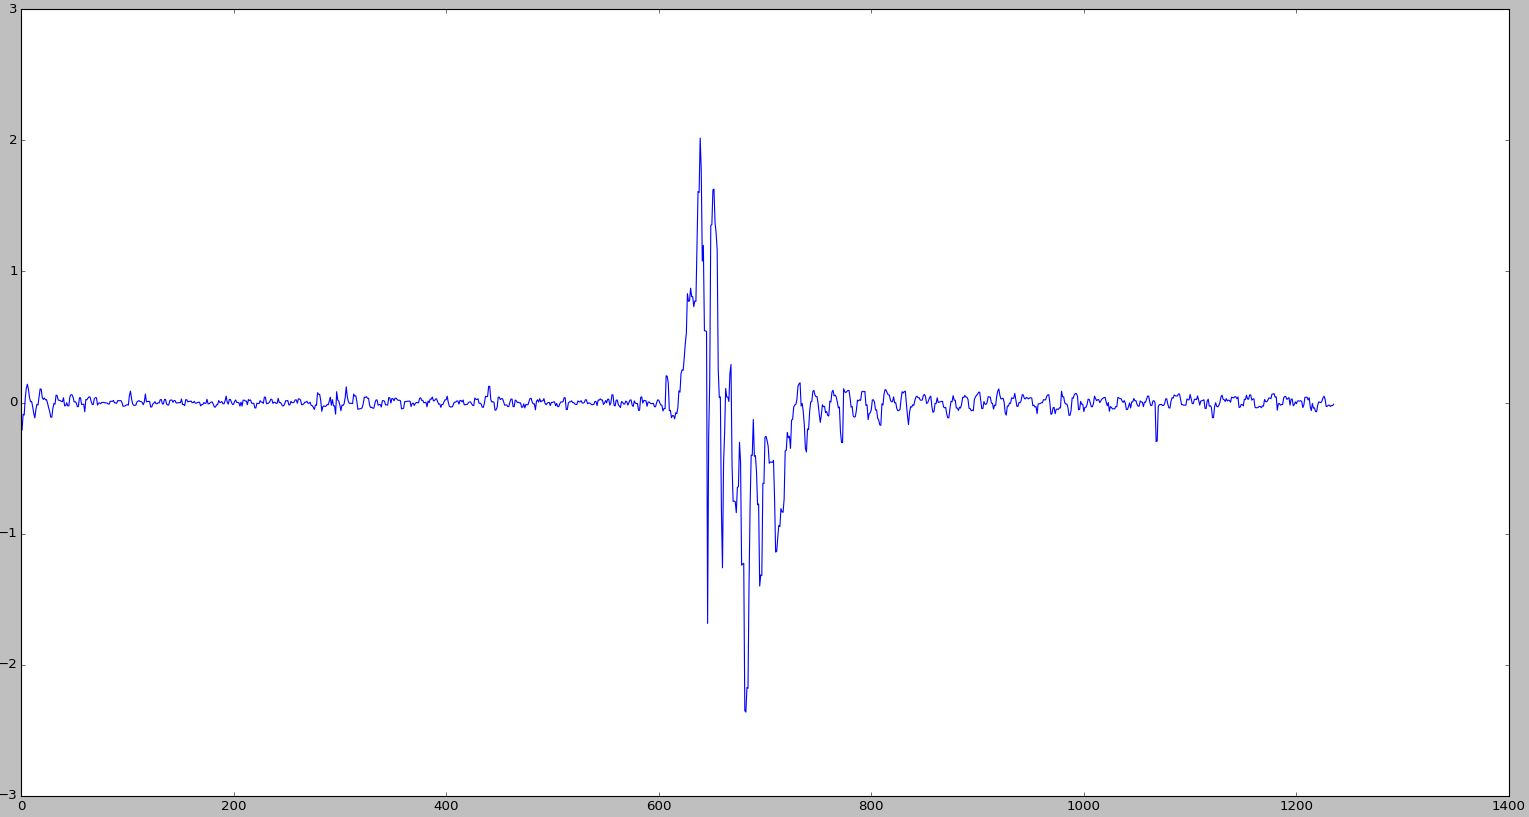
\includegraphics[width=1.0\linewidth]{rawacc.jpg}
					  	\caption{}
					  	\label{fig:sub1}
					\end{subfigure}%
					\begin{subfigure}{.5\textwidth}
					  	\centering
					  	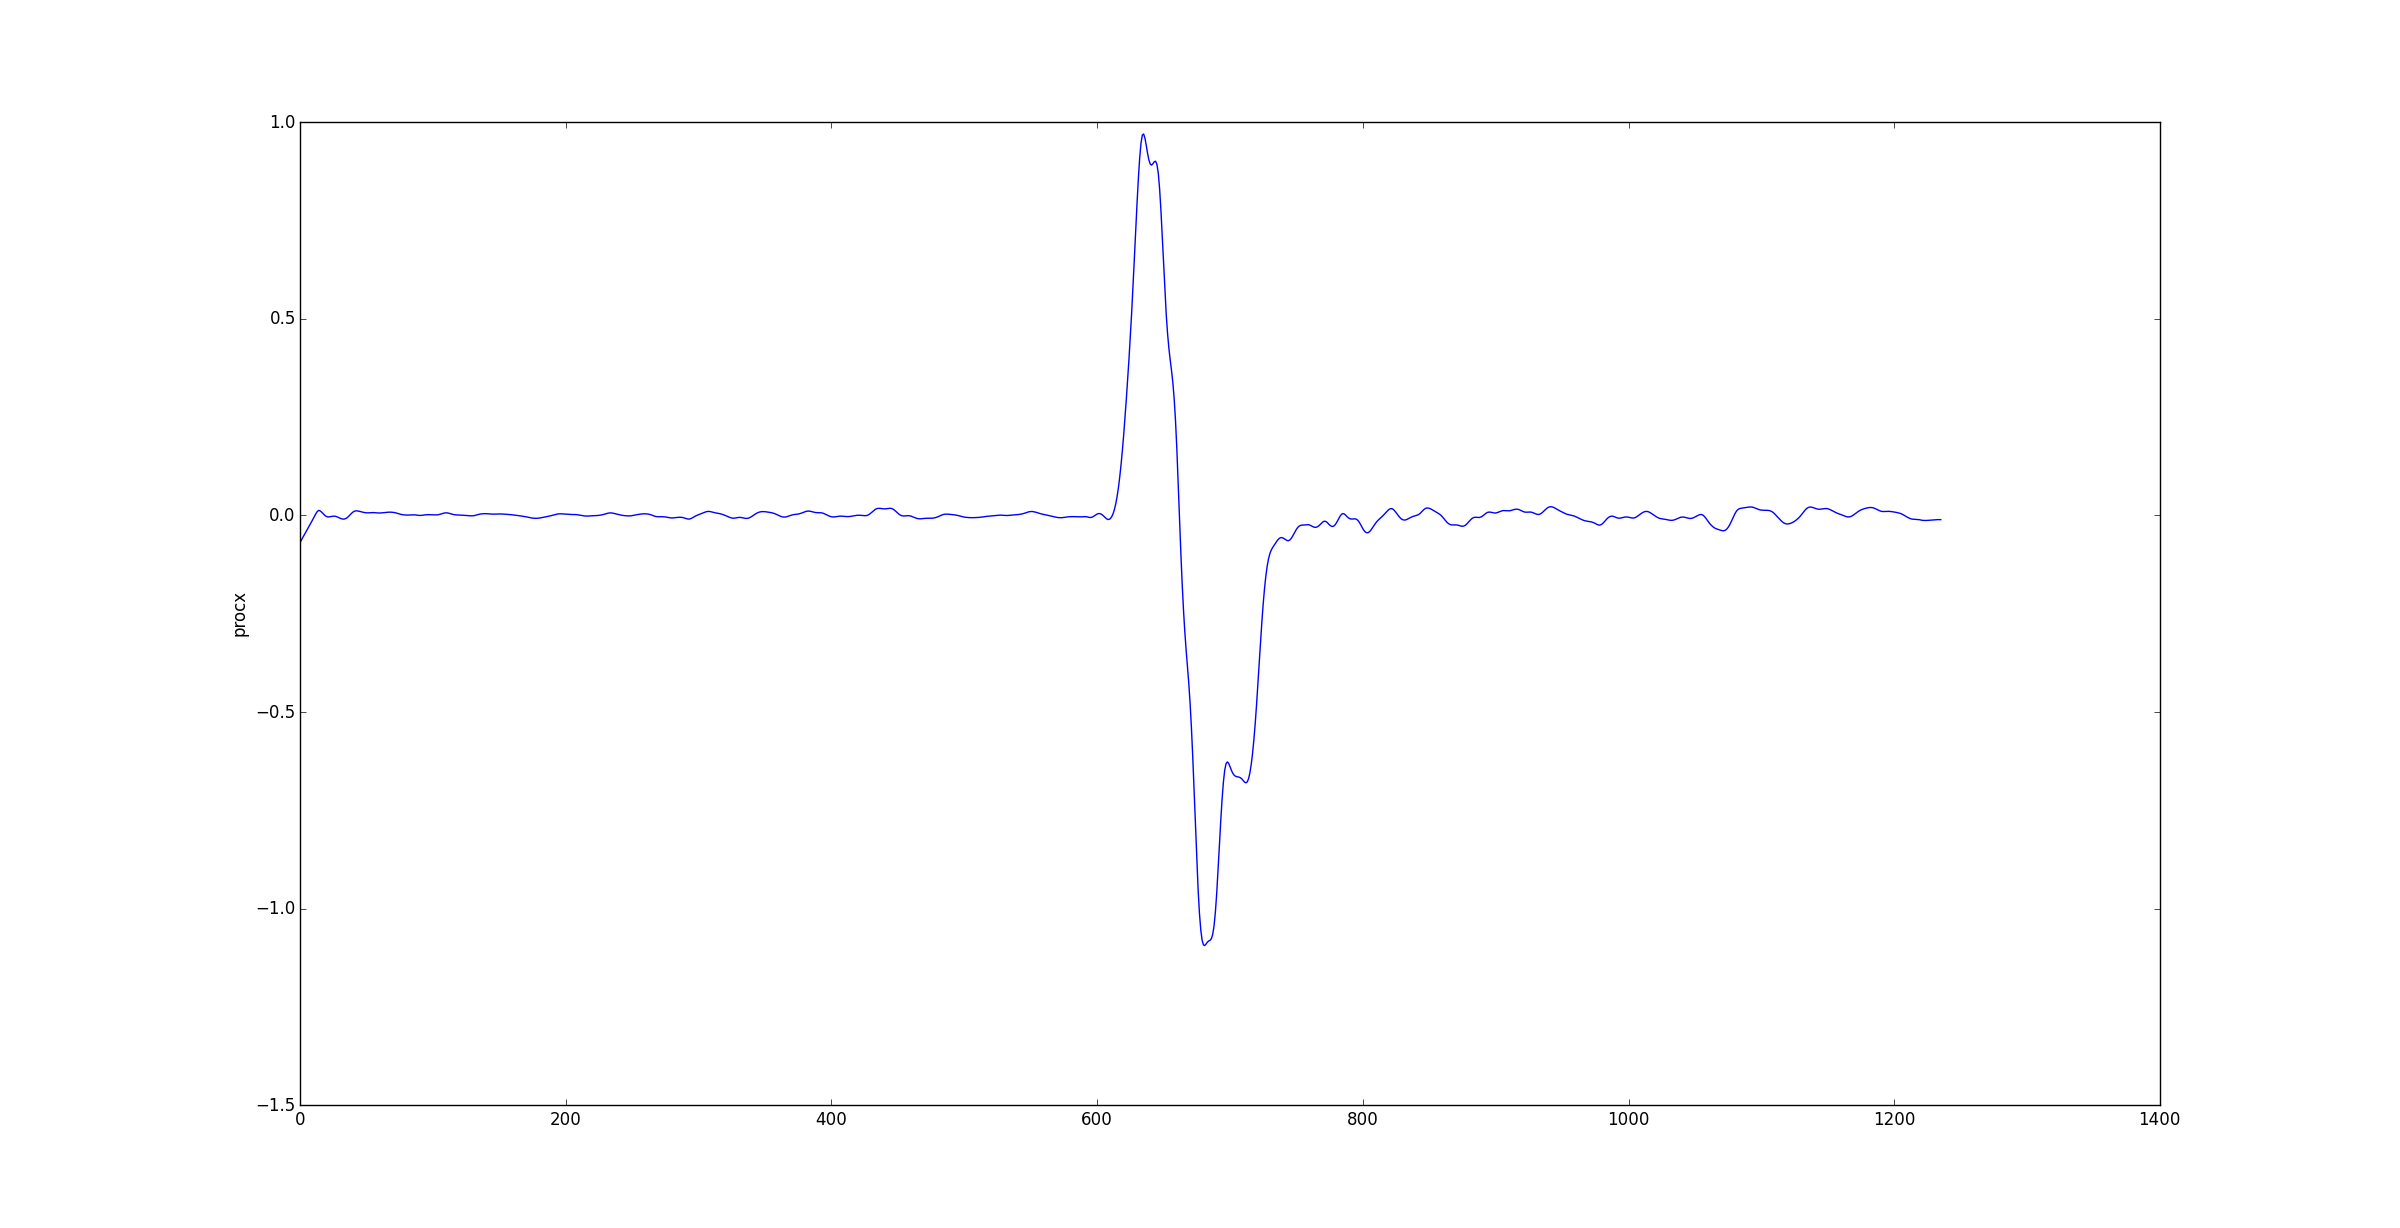
\includegraphics[width=1.0\linewidth]{procacc.jpg}
					  	% \caption{Dense reconstruction}
					  	\caption{}
					  	\label{fig:sub2}
					\end{subfigure}
					\caption{Acceleration Smoothening}
					\label{figstart}
			\end{figure}
			The second graph has smoothened the kinks in the first graph thus our procedure is very successful in removing noise from raw acceleration data.

			\item Figure 4 shows two graph represents the value of distance obtained direct integration and our procedure for 30cm movmement for different trials
				\begin{figure}[H]
					\centering
					\begin{subfigure}{.5\textwidth}
					  	\centering
					  	\includegraphics[width=1.0\linewidth]{simpleInt.jpg}
					  	\caption{}
					  	\label{fig:sub1}
					\end{subfigure}%
					\begin{subfigure}{.5\textwidth}
					  	\centering
					  	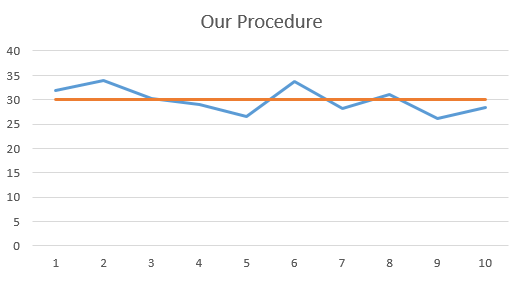
\includegraphics[width=1.0\linewidth]{ourproc.jpg}
					  	% \caption{Dense reconstruction}
					  	\caption{}
					  	\label{fig:sub2}
					\end{subfigure}
					\caption{Distance Estimations}
					\label{figstart}
			\end{figure}
			The above graphs show that our procedure clearly gives more reliable results.

			\item Figure 5 shows a graph which represents the value of rotation obtained from our procedure against various ground truths.
				   \begin{figure}
    			  % \begin{subfigure}{.5\textwidth}
    			      \centering
    			      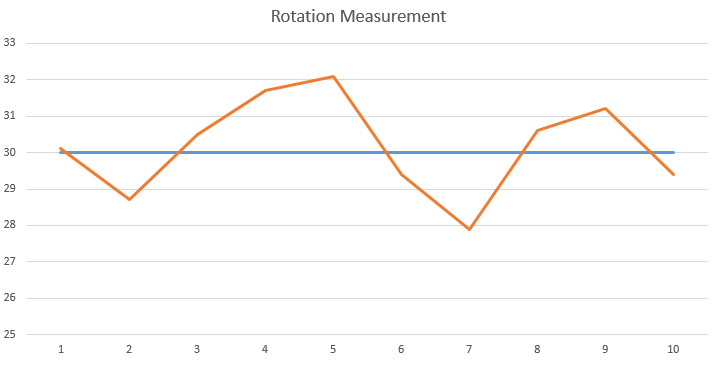
\includegraphics[width=0.55\linewidth]{rot.jpg}
    			      \caption{Rotation Values}
    			      % \label{fig:sub2}
    			  % \end{subfigure}
    			  % \caption{3D reconstruction}
    			  % \label{figstart}
    			\end{figure}
    		As can be seen from the graph, that the values obtained are very close to the ground truth. Thus, this shows that our procedure is highly accurate.
    		

			\item Figure 6 shows a graph identifying the motion zone using our procedure.
			   \begin{figure}
    			  % \begin{subfigure}{.5\textwidth}
    			      \centering
    			      \includegraphics[width=0.55\linewidth]{motzone.jpg}
    			      \caption{Motion Zones}
    			      % \label{fig:sub2}
    			  % \end{subfigure}
    			  % \caption{3D reconstruction}
    			  % \label{figstart}
    			\end{figure}
    		The detection of the motion zone is highly accurate and efficient using our procedure

			\end{itemize} 

		\vspace{3mm}
		\
			\section{Generating point correspondences}
		We exploited the video feed from the camera to generate correspondences through visual tracking of points. It was done in the following way.
		\begin{enumerate}
			\item Feature points were identified in the first frame using Good features to track.
			\item These points were tracked in the following video frame using sparse optical flow (KL Tracker)
			\item As a result, from the first frame a chain of points was established till the next image was captured and hence correspondences were identified.
			\item Due to quick movement taking place, the number of tracked points would drop. To ensure that this is corrected, more feature points were added after every 10 frames so that enough points are available.
		\end{enumerate}
		\subsection{Results}
			\begin{itemize}
				\item The above procedure works in real time on the device.
				\item The correspondences obtained are multi image correspondences. 
				\item To identify the frame rate required for this method to work, an off-line program was run on various frame rates. It was seen that frame rate above 6-7 was able to produce accurate correspondences.
				\item The average number of correspondences obtained from a dataset of images is as follows: \\ 
					\begin{center}
 					\begin{tabular}{|c | c|}
 						\hline
 						Number of Images & Average Number of Correspondences \\ \hline
 						2 & TODO \\ \hline
 						3 & TODO \\ \hline
 						4 & TODO \\ \hline
 						5 & TODO \\ \hline
 						6 & TODO \\ \hline
 						7 & TODO \\ \hline
 						8 & TODO \\ \hline

					\end{tabular}
					\end{center}
				\item The quality and number of correspondences can be improved by incorporating a kalman filter to allow points dropped in a frame to re enter the procedure.
				\item The correspondences obtained contain some errors which can be seen in the following:
				    \begin{figure}[ht!]
			      \centering
          				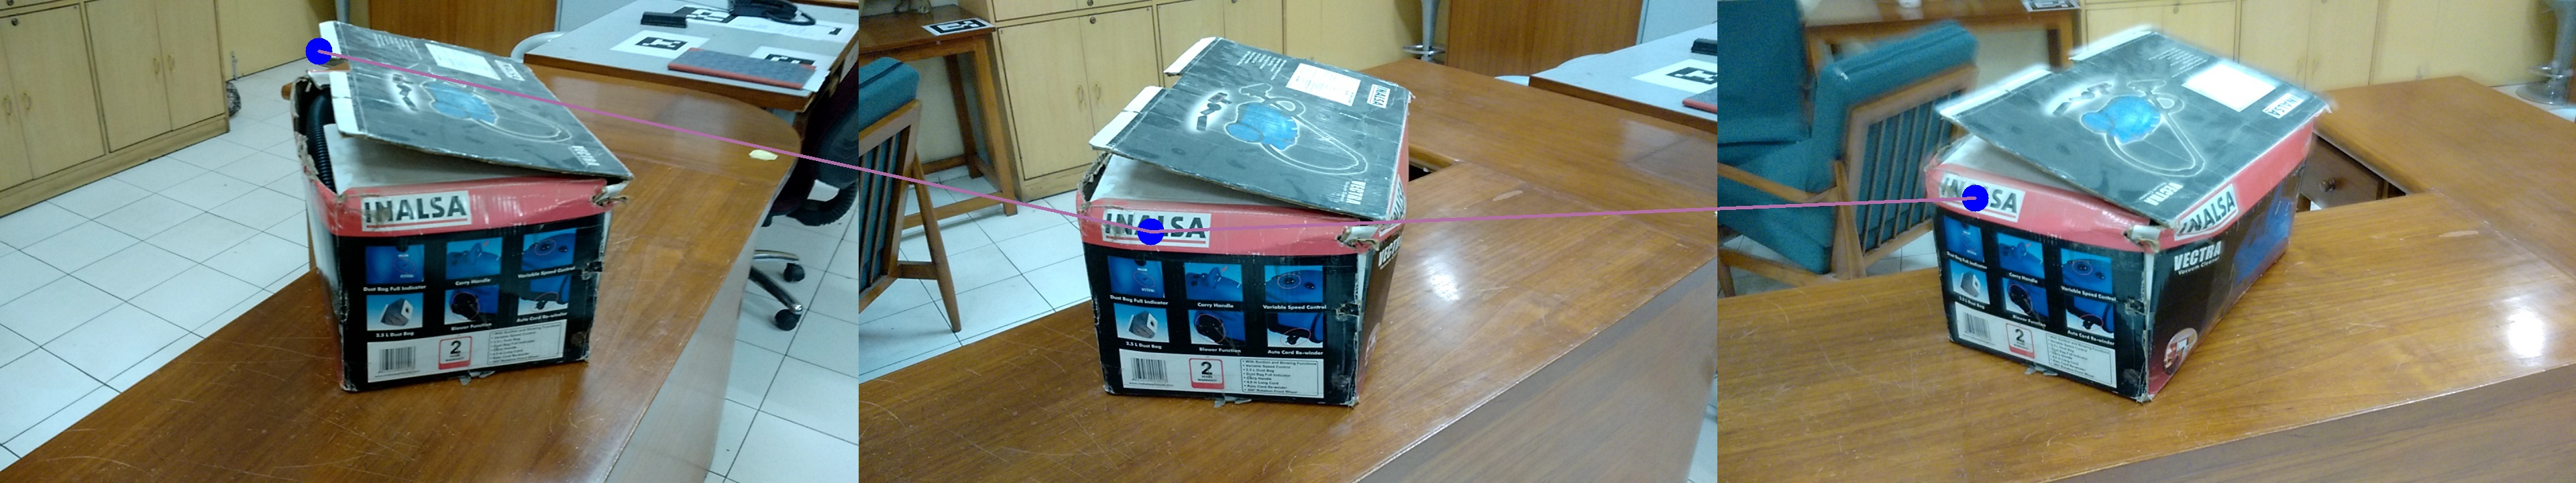
\includegraphics[width=1.0\linewidth]{00018.jpg}
          				\caption{Incorrect Correspondence}
          % \label{fig:sub1}
      % \end{subfigure}%
    \end{figure}
    \begin{figure}
      % \begin{subfigure}{.5\textwidth}
          \centering
          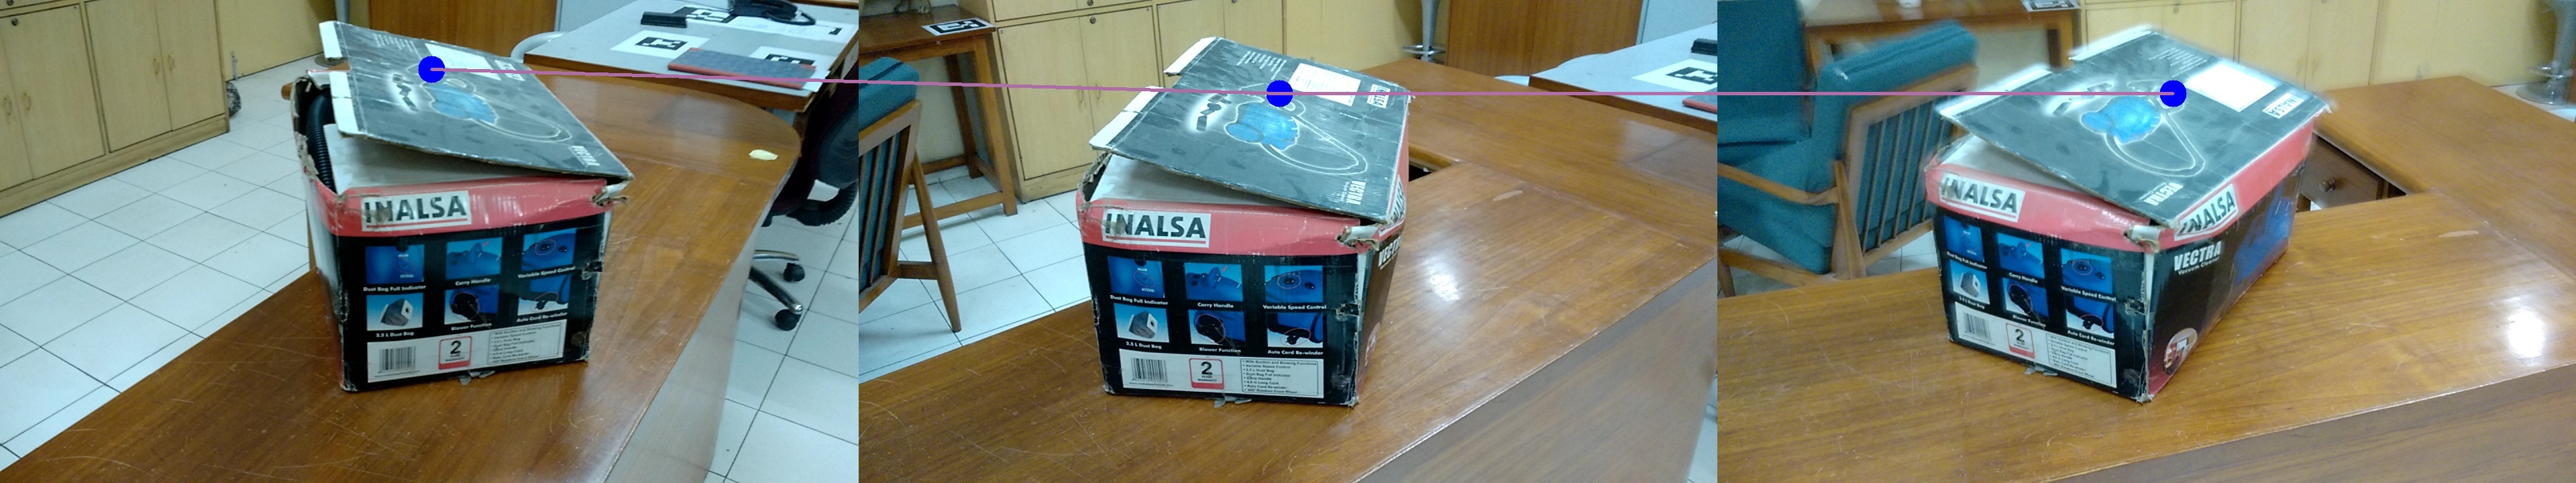
\includegraphics[width=1.0\linewidth]{00027.jpg}
          \caption{Correct Correspondence}
          % \label{fig:sub2}
      % \end{subfigure}
      % \caption{3D reconstruction}
      % \label{figstart}
    \end{figure}
			\end{itemize}
		% \\
		% \vspace{6mm}

	\newpage
	\section{3D Reconstruction}
		Using the correspondences and position orientation data obtained previously, 3D reconstruction is performed.
		\begin{enumerate}
		\item Conversion the Orientation Matrix (Mobile Sensors Frame) to Rotation Matrix (Camera Frame) \\
			  \begin{equation}
   				\mathbf{R}  = 
				    \begin{bmatrix}
				    1 & 0 & 0 \\ 0 & -1 & 0 \\ 0 & 0 & 1  
				    \end{bmatrix} *
				    \begin{bmatrix}
				    0 & 1 & 0 \\ -1 & 0 & 0 \\ 0 & 0 & 1 
				    \end{bmatrix} *
				    \begin{bmatrix}
				    R_0 & R_1 & R_2 \\ R_3 & R_4 & R_5 \\
				    R_6 & R_7 & R_8 
				    \end{bmatrix}
			  \end{equation} \\
			\begin{itemize}
			\item The first matrix brings a flip of the y axis.
			\item The second matrix aligns the x and z axis of the frame of sensors with the camera frame.
			\end{itemize}
		\item Conversion of Position Matrix to Translation Matrix \\ 
			\begin{equation}
				\mathbf{T} = - \mathbf{R} * \mathbf{C}
 			\end{equation} \\
 			The above equation changes the position of the camera in ground frame to the translation in the frame of the image.
		\item Triangulation \\
			\begin{itemize}
				\item The intrinsic camera matrix is precomputed from the focal length of the camera. For the case of Xiaomi Mi4 the matrix is as follows: \\ 
					\begin{equation}
						\mathbf{K} = \begin{bmatrix} 8.695*10^{-4} & 0 & 0 \\
						0 & 8.695*10^{-4} & 0 \\ 0 & 0 & 1 \end{bmatrix} 
					\end{equation}
				\item Using equation 1 and the R, T, K matrices for a given set of corresponding points, a system of linear equations is solved to obtain the 3D coordinates of the point.   
			\end{itemize}
		\item Bundle Adjustment \\
			After the triangulation has taken place from the estimated R,T matrices, a bundle adjustment is done to improve the 3D point coordinates, rotation and translation matrices to yield the final result. 
		\end{enumerate}
		\subsection{Results}
			\begin{enumerate}
				\item The accuracy of the rotation and translation matrix obtained from the IMU sensors compared against the R,T matrix obtained from computer vision techniques is as follows:
				 % \begin{center}
	\\ 					\begin{tabular}{|c | c | c | c |}
 						\hline
 						S.No. & No. of Images & Avg. Error in Translation & Avg. Error in Rotation \\ \hline
 						1 & TODO & TODO & TODO \\ \hline
 						2 & TODO & TODO & TODO \\ \hline
 						3 & TODO & TODO & TODO \\ \hline
 						4 & TODO & TODO & TODO \\ \hline
 						5 & TODO & TODO & TODO \\ \hline
 						6 & TODO & TODO & TODO \\ \hline
 						7 & TODO & TODO & TODO \\ \hline
					\end{tabular}
				\item Consider the images shown
				\begin{figure}[H]
					\centering
					\begin{subfigure}{.33\textwidth}
					  	\centering
					  	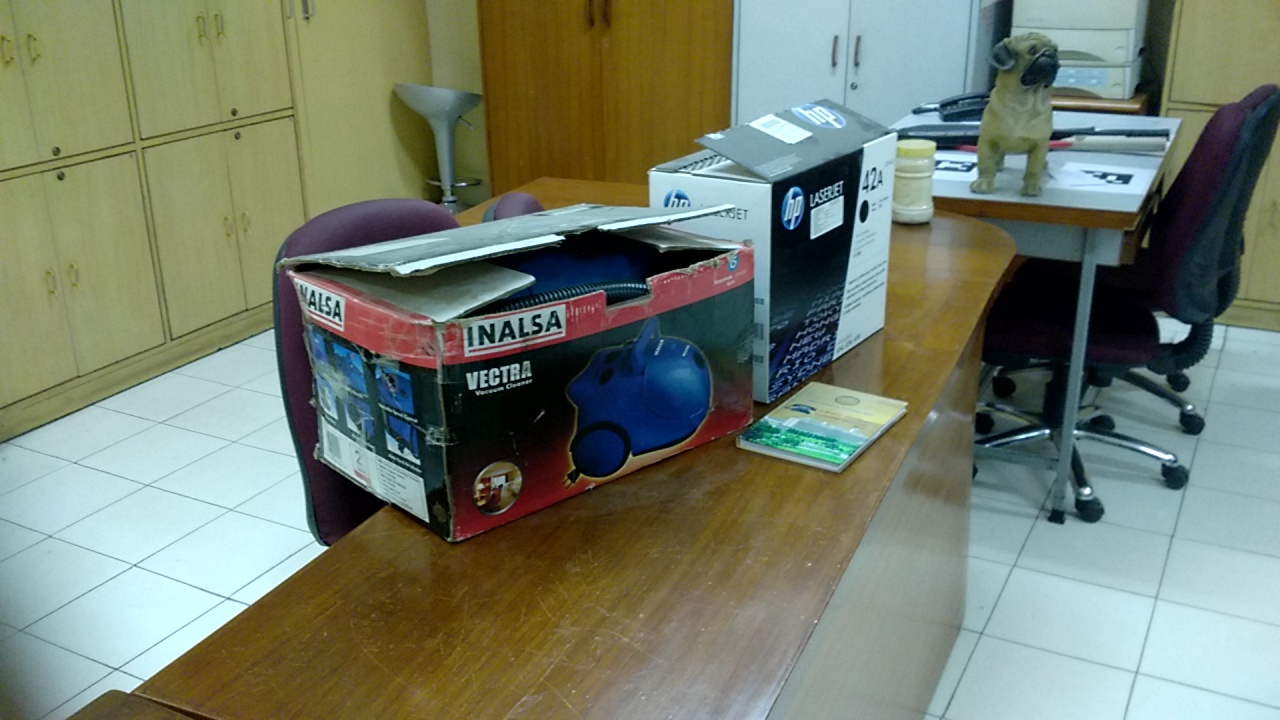
\includegraphics[width=1.0\linewidth]{1_0_image.jpg}
					  	\caption{}
					  	\label{fig:sub1}
					\end{subfigure}%
					\begin{subfigure}{.33\textwidth}
					  	\centering
					  	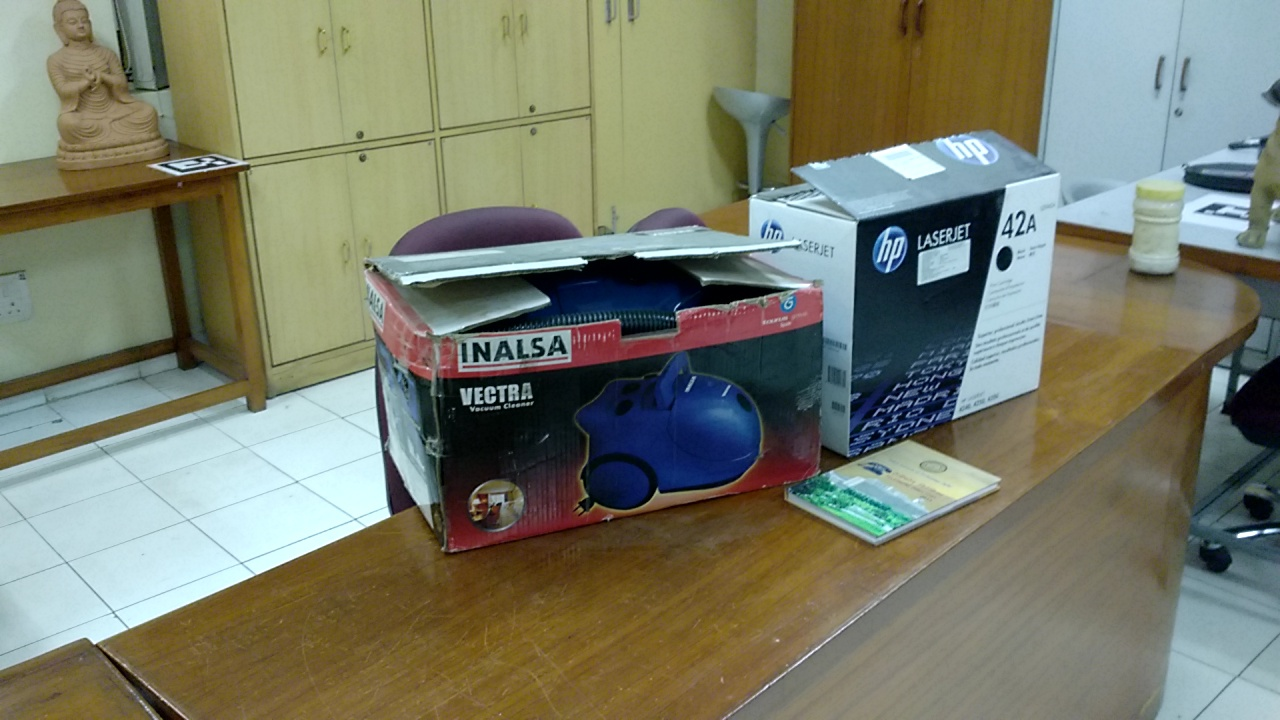
\includegraphics[width=1.0\linewidth]{1_1_image.jpg}
					  	% \caption{Dense reconstruction}
					  	\caption{}
					  	\label{fig:sub2}
					\end{subfigure}
					\begin{subfigure}{.33\textwidth}
					  	\centering
					  	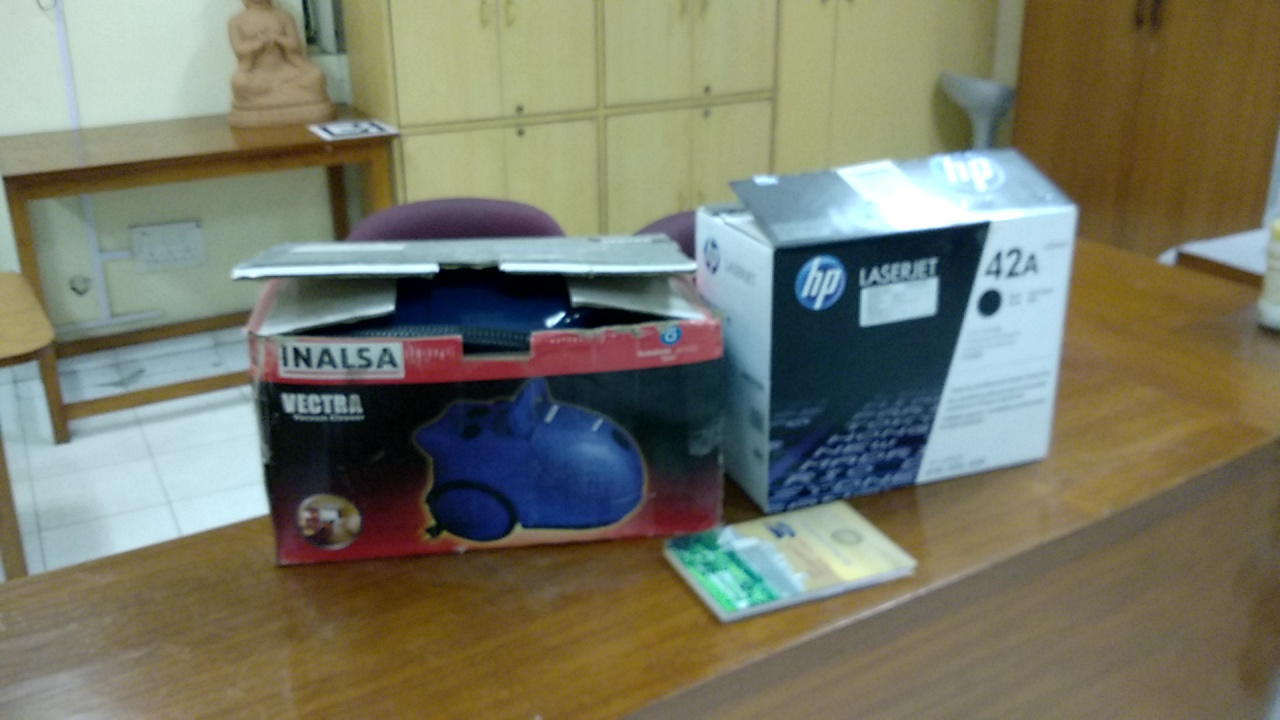
\includegraphics[width=1.0\linewidth]{1_2_image.jpg}
					  	% \caption{Dense reconstruction}
					  	\caption{}
					  	\label{fig:sub2}
					\end{subfigure}
					% \\ 
					\begin{subfigure}{.33\textwidth}
					  	\centering
					  	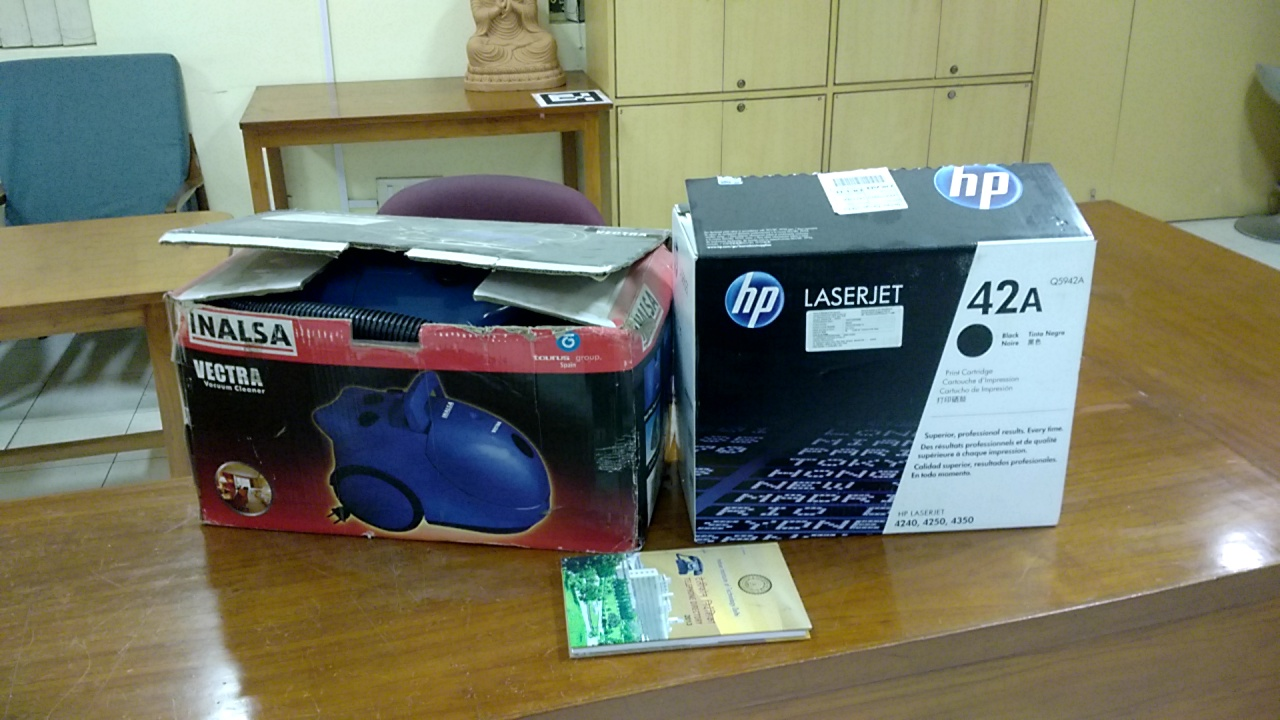
\includegraphics[width=1.0\linewidth]{1_3_image.jpg}
					  	% \caption{Sparse reconstruction}
					  	
					  	\caption{}\label{fig:sub1}
					\end{subfigure}%
					\begin{subfigure}{.33\textwidth}
					  	\centering
					  	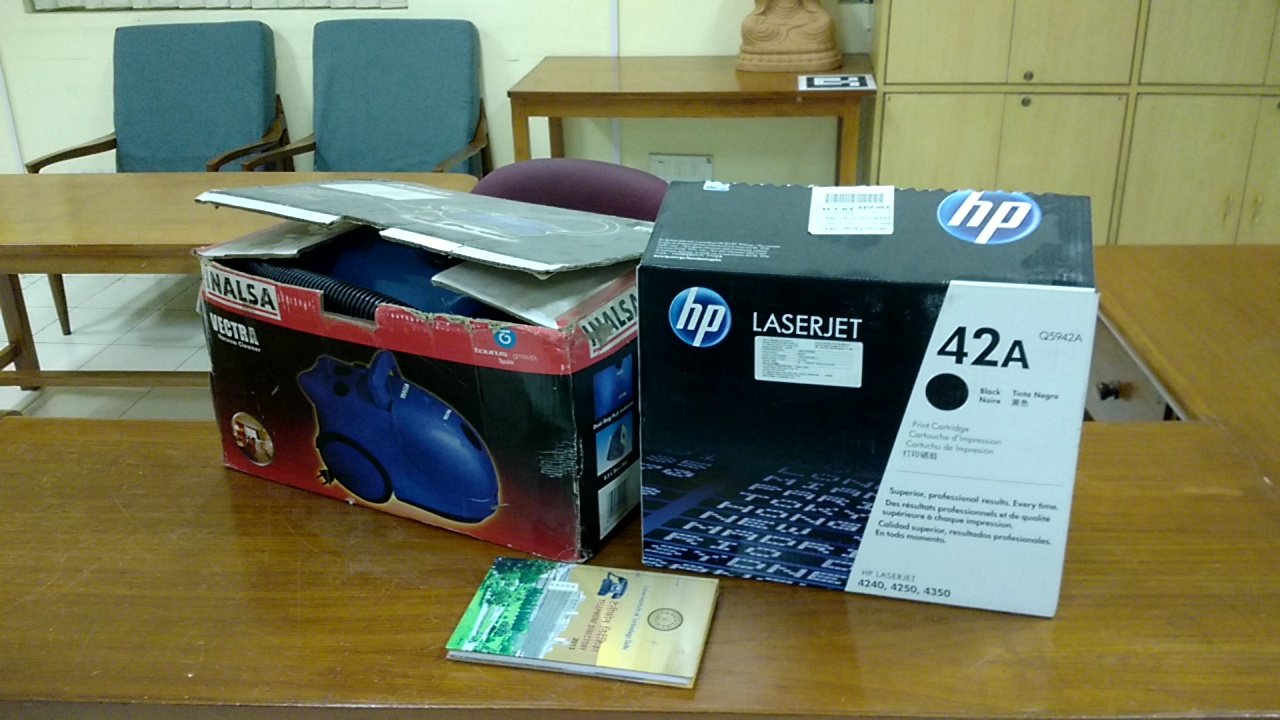
\includegraphics[width=1.0\linewidth]{1_4_image.jpg}
					  	% \caption{Dense reconstruction}
					  	\caption{}\label{fig:sub2}
					\end{subfigure}
					\begin{subfigure}{.33\textwidth}
					  	\centering
					  	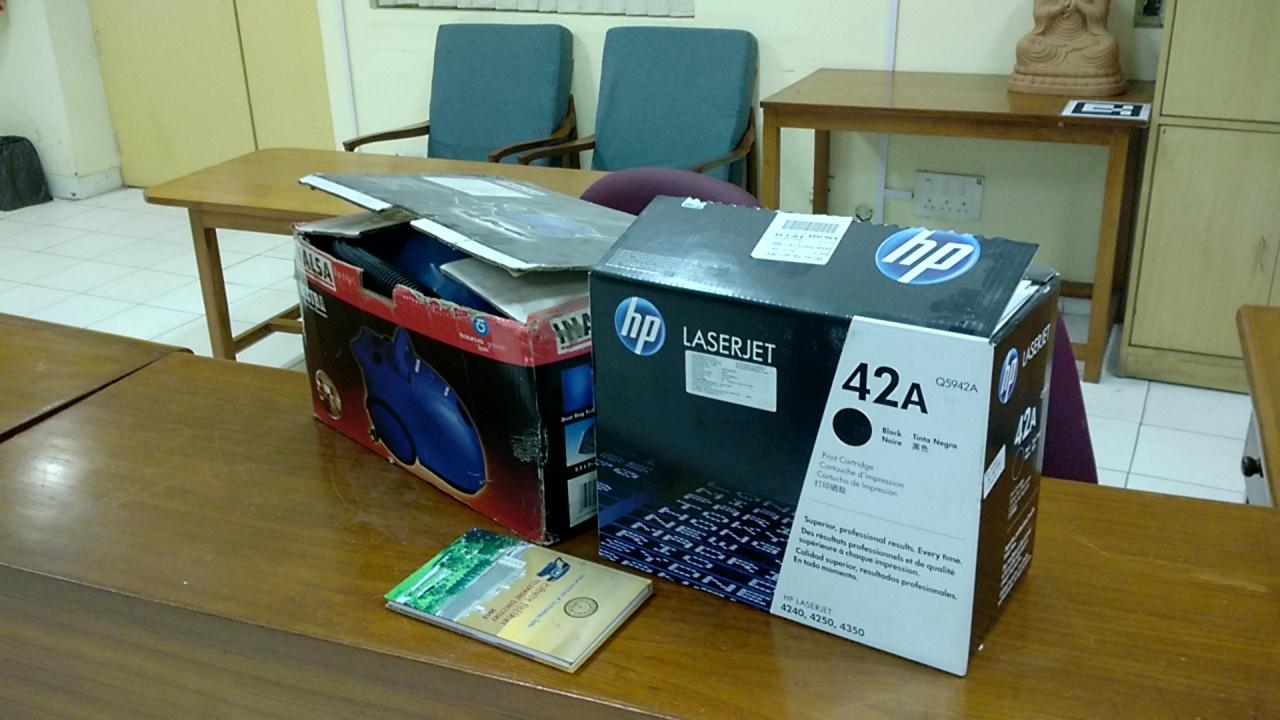
\includegraphics[width=1.0\linewidth]{1_5_image.jpg}
					  	% \caption{Dense reconstruction}
					  	\caption{}\label{fig:sub2}
					\end{subfigure}
					% \caption{Images}
					
					% \\
					\begin{subfigure}{.7\textwidth}
					  	\centering
					  	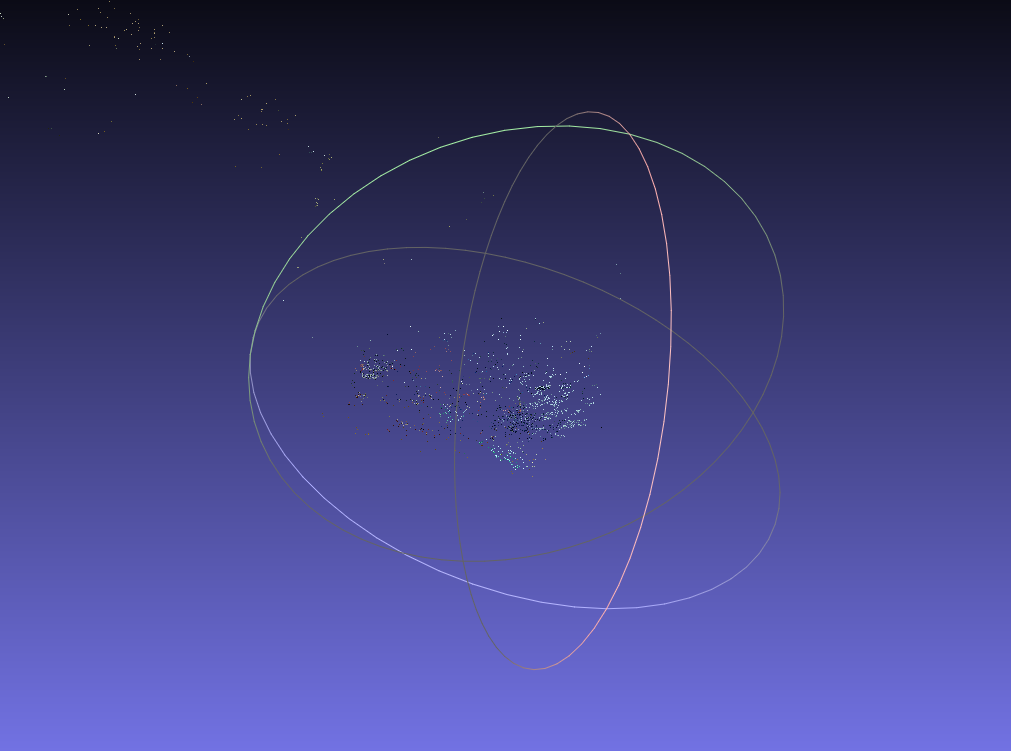
\includegraphics[width=1.0\linewidth]{1_sensors.png}
					  	\caption{Reconstruction from sensors}
					  	\label{fig:sub2}
					\end{subfigure}
					\begin{subfigure}{.7\textwidth}
					  	\centering
					  	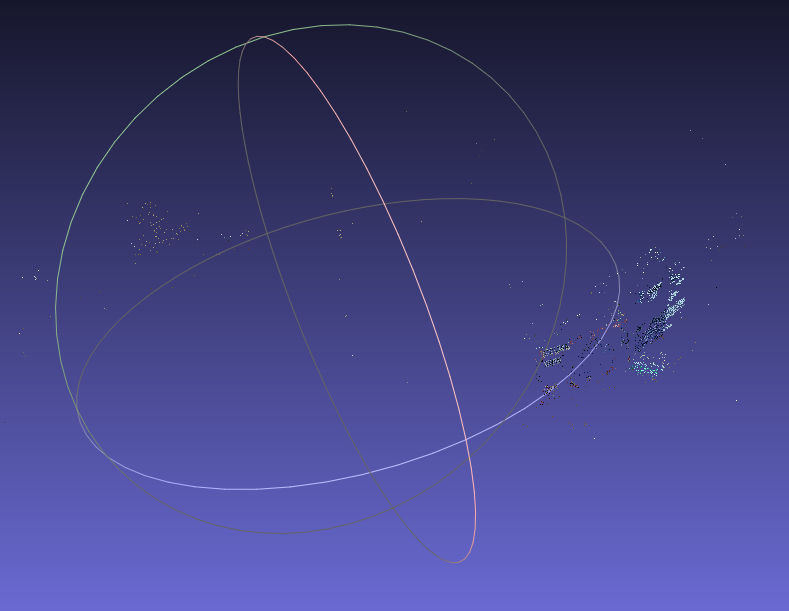
\includegraphics[width=1.0\linewidth]{1_bundler.png}
					  	\caption{Bundle Adjustment}
					  	\label{fig:sub2}
					\end{subfigure}
					\caption{Images}
					\label{figstart}


			\end{figure}
					\begin{itemize}
						\item Figures a-f capture the images of 2 boxes placed on a table from different positions
						\item Figure g is the output of triangulation using the information obtained from tracking and sensors. The points can be seen to represent a rough structure of the boxes shown in the images. Different set of layers can be observed which are supposed to represent the same flat surface.
						\item After running bundle adjustment, the 3D structure of the boxes can be visualized clearly in Figure h 
					\end{itemize}	
			\end{enumerate}
	\section{References}

\end{document}